\documentclass[orivec]{llncs}
\usepackage{graphicx}
\usepackage{amsmath}			% for "cases"
\usepackage{amsfonts}		% for frakur fonts
\usepackage{mathrsfs}		% for curly "E" error symbol
\usepackage{float}
\usepackage{tcolorbox}		% for wrapping example in color box
\usepackage{wrapfig}			% wrap figure beside text, used in example
\usepackage{tikz-cd}			% commutative diagrams
\usepackage{amssymb}			% for \multimap, \updownarrow, \bigstar
\usepackage{sectsty}			% change section color
\usepackage{turnstile}		% longer turnstiles
\usepackage{hyperref}		% include web link for RL sample code

\usepackage{geometry}		% change paper size
\geometry{
  a4paper,         % or letterpaper
  textwidth=18cm,  % llncs has 12.2cm
  textheight=27cm, % llncs has 19.3cm
  heightrounded,   % integer number of lines
  hratio=1:1,      % horizontally centered
  vratio=2:3,      % not vertically centered
}
\usepackage[fontsize=13pt]{scrextend}

% *************** Delete when not using Chinese or colors **********************
\usepackage{xeCJK}
\setCJKmainfont[BoldFont=SimHei,ItalicFont=KaiTi]{SimSun}
\usepackage{color}
\definecolor{Cerulean}{RGB}{100,100,200}
\newcommand{\emp}[1]{\textbf{\textcolor{Cerulean}{#1}}}
\definecolor{grey}{rgb}{0.9,0.9,0.9}  % grey

% \chapterfont{\color{blue}}  % sets colour of chapters
\sectionfont{\color{blue}} 
\subsectionfont{\color{blue}} 
\subsubsectionfont{\color{blue}} 

\newcommand{\vect}[1]{\boldsymbol{#1}}
\newcommand*\sigmoid{\vcenter{\hbox{
\includegraphics{sigmoid.png}}}}
\newcommand*\KB{\vcenter{\hbox{
\includegraphics{KB-symbol.png}}}}
\newcommand*\invsigmoid{\vcenter{\hbox{
\includegraphics{inverse-sigmoid.png}}}}
\newcommand{\invW}{\, \rotatebox[origin=c]{90}{W}}
\newcommand{\invw}{\, \rotatebox[origin=c]{90}{w}}
\newcommand*\rectifier{\vcenter{\hbox{
\includegraphics{rectifier.png}}}}
\newcommand{\dashh}{\textemdash~}
\newcommand{\code}[1]{{\footnotesize{\ttfamily #1}}}
\newcommand{\tab}{\hspace*{1cm} }

% ***** Boxed variables inside math equations
% \newcommand*{\boxedcolor}{black}
\makeatletter
% \renewcommand{\boxed}[1]{\textcolor{\boxedcolor}{%
% \fbox{\normalcolor\m@th$\displaystyle#1$}}}
% \setlength{\fboxsep}{1pt}
\renewcommand{\boxed}[1]{\fbox{\m@th$\displaystyle\scalebox{0.9}{#1}$} \,}
\makeatother

\overfullrule=0mm

\newsavebox{\MyName}
\savebox{\MyName}{
\includegraphics[scale=0.6]{YKY.png}}

\title{游荡在思考的迷宫中}
\titlerunning{游荡在思考的迷宫中}
\author{King-Yin Yan (\usebox{\MyName})
% \\ \footnotesize{General.Intelligence@Gmail.com}
\and
Ben Goertzel
\and
Juan Carlos Kuri Pinto
}
\institute{General.Intelligence@Gmail.com}

\begin{document}

\maketitle
\setlength{\parindent}{0em}
% \setlength{\parskip}{2.8ex plus0.8ex minus0.8ex}
\setlength{\parskip}{2.8ex}

\begin{abstract}
介绍一个基於 \textbf{增强学习} 和 \textbf{深度学习} 的极简约的 cognitive architecture,它在数学上是一个Hamiltonian 系统,而其 Lagrangian 对应於智能系统的「奖励」或「欲望」的价值。 经典逻辑 AI 的技巧可以搬到这个 setting 之下,而连续时间化之后,可以用上微分几何的技巧。 
% 简单介绍笔者的强人工智能理论和强化学习、动态规划、最优控制、
% 假设 $x$ 是思维状态。 在经典逻辑智能中,$x$ 是一束命题,代表当下的思考状况。 思考的过程就是不断重复进行推导: $x \vdash x' \vdash ...$。 在经典 AI 中这个作用是靠无数的逻辑 rules 来达成的。 但现在我们的做法是将 $x$ 放到向量空间中,再用一个 recurrent 神经网络来取代整个 rules base。
\end{abstract}

本文较少原创内容,主要介绍一些已知的理论,及提供一个新的观点,或许对 strong AI 的发展有帮助。

\setcounter{section}{-1}
\section{中心思想}

标题中的\textbf{比喻}是指用增强学习的方法控制一隻自主的智能系统 (autonomous agent),在「思维空间」中寻找最优路径:
\begin{equation}
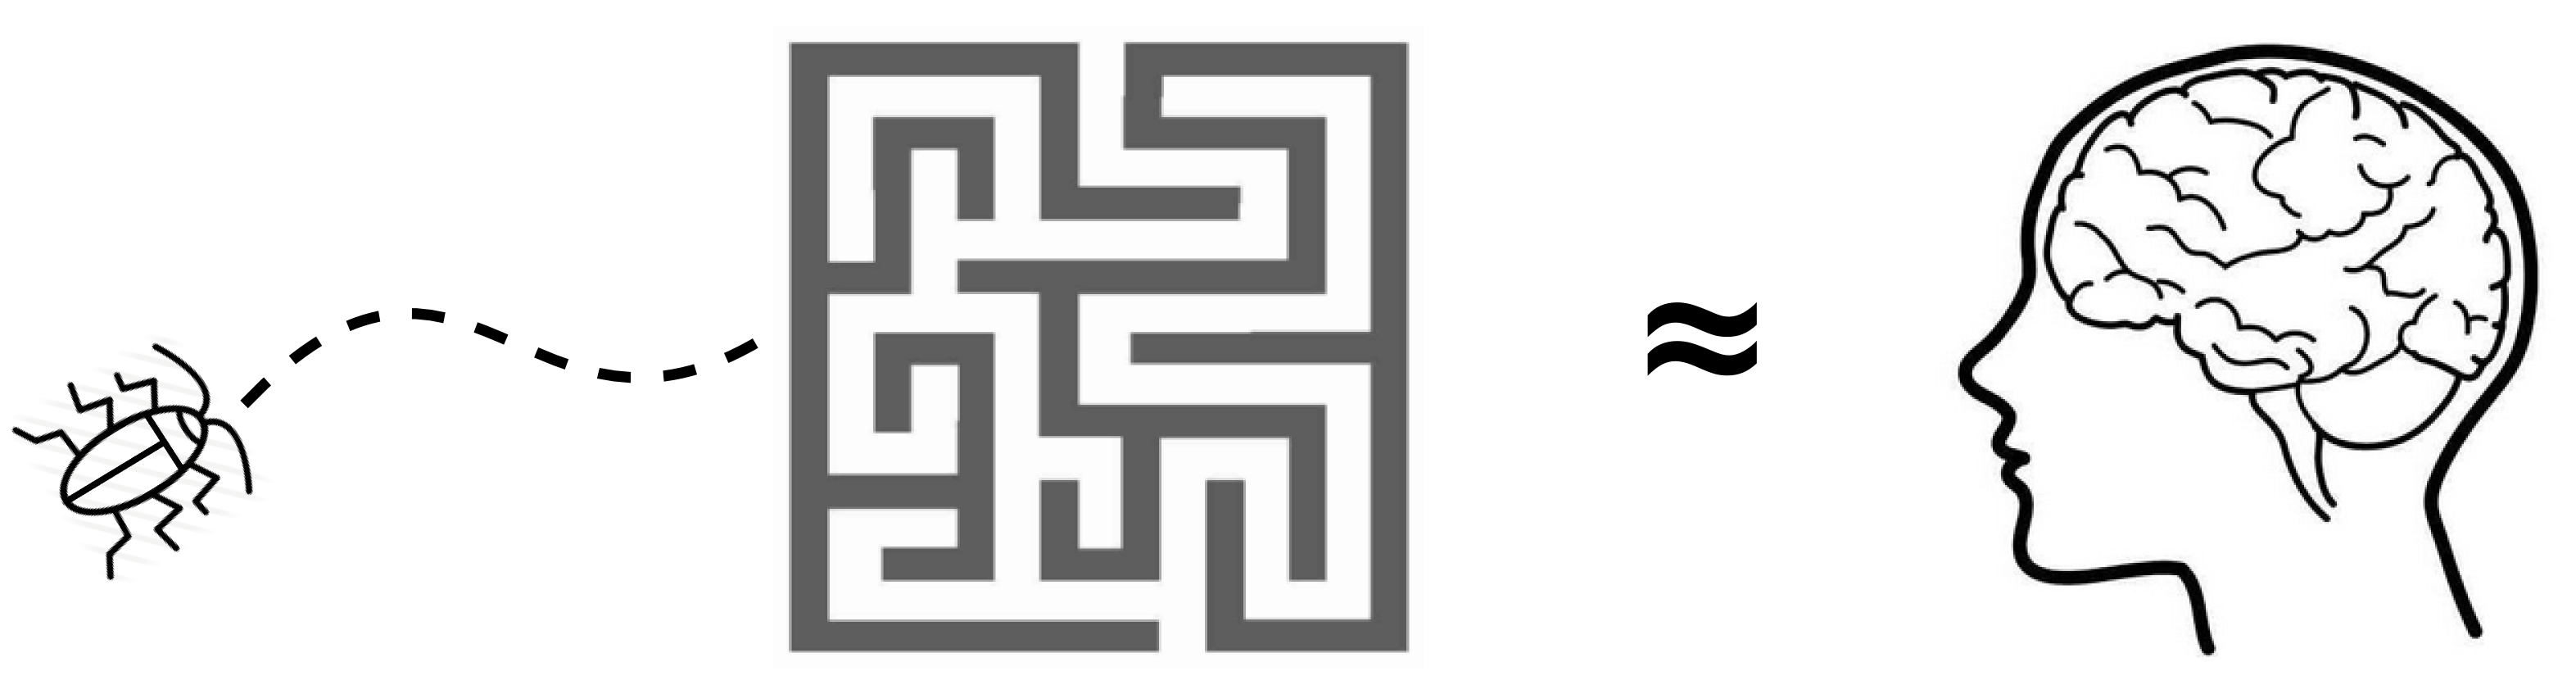
\includegraphics[scale=0.65]{maze-metaphor.png}
\end{equation}

关键是将「思考」看成是一个\emp{动态系统} (dynamical system),它运行在\emp{思维状态} (mental states) 的空间中:
\begin{equation}
\label{fig:mental-state}
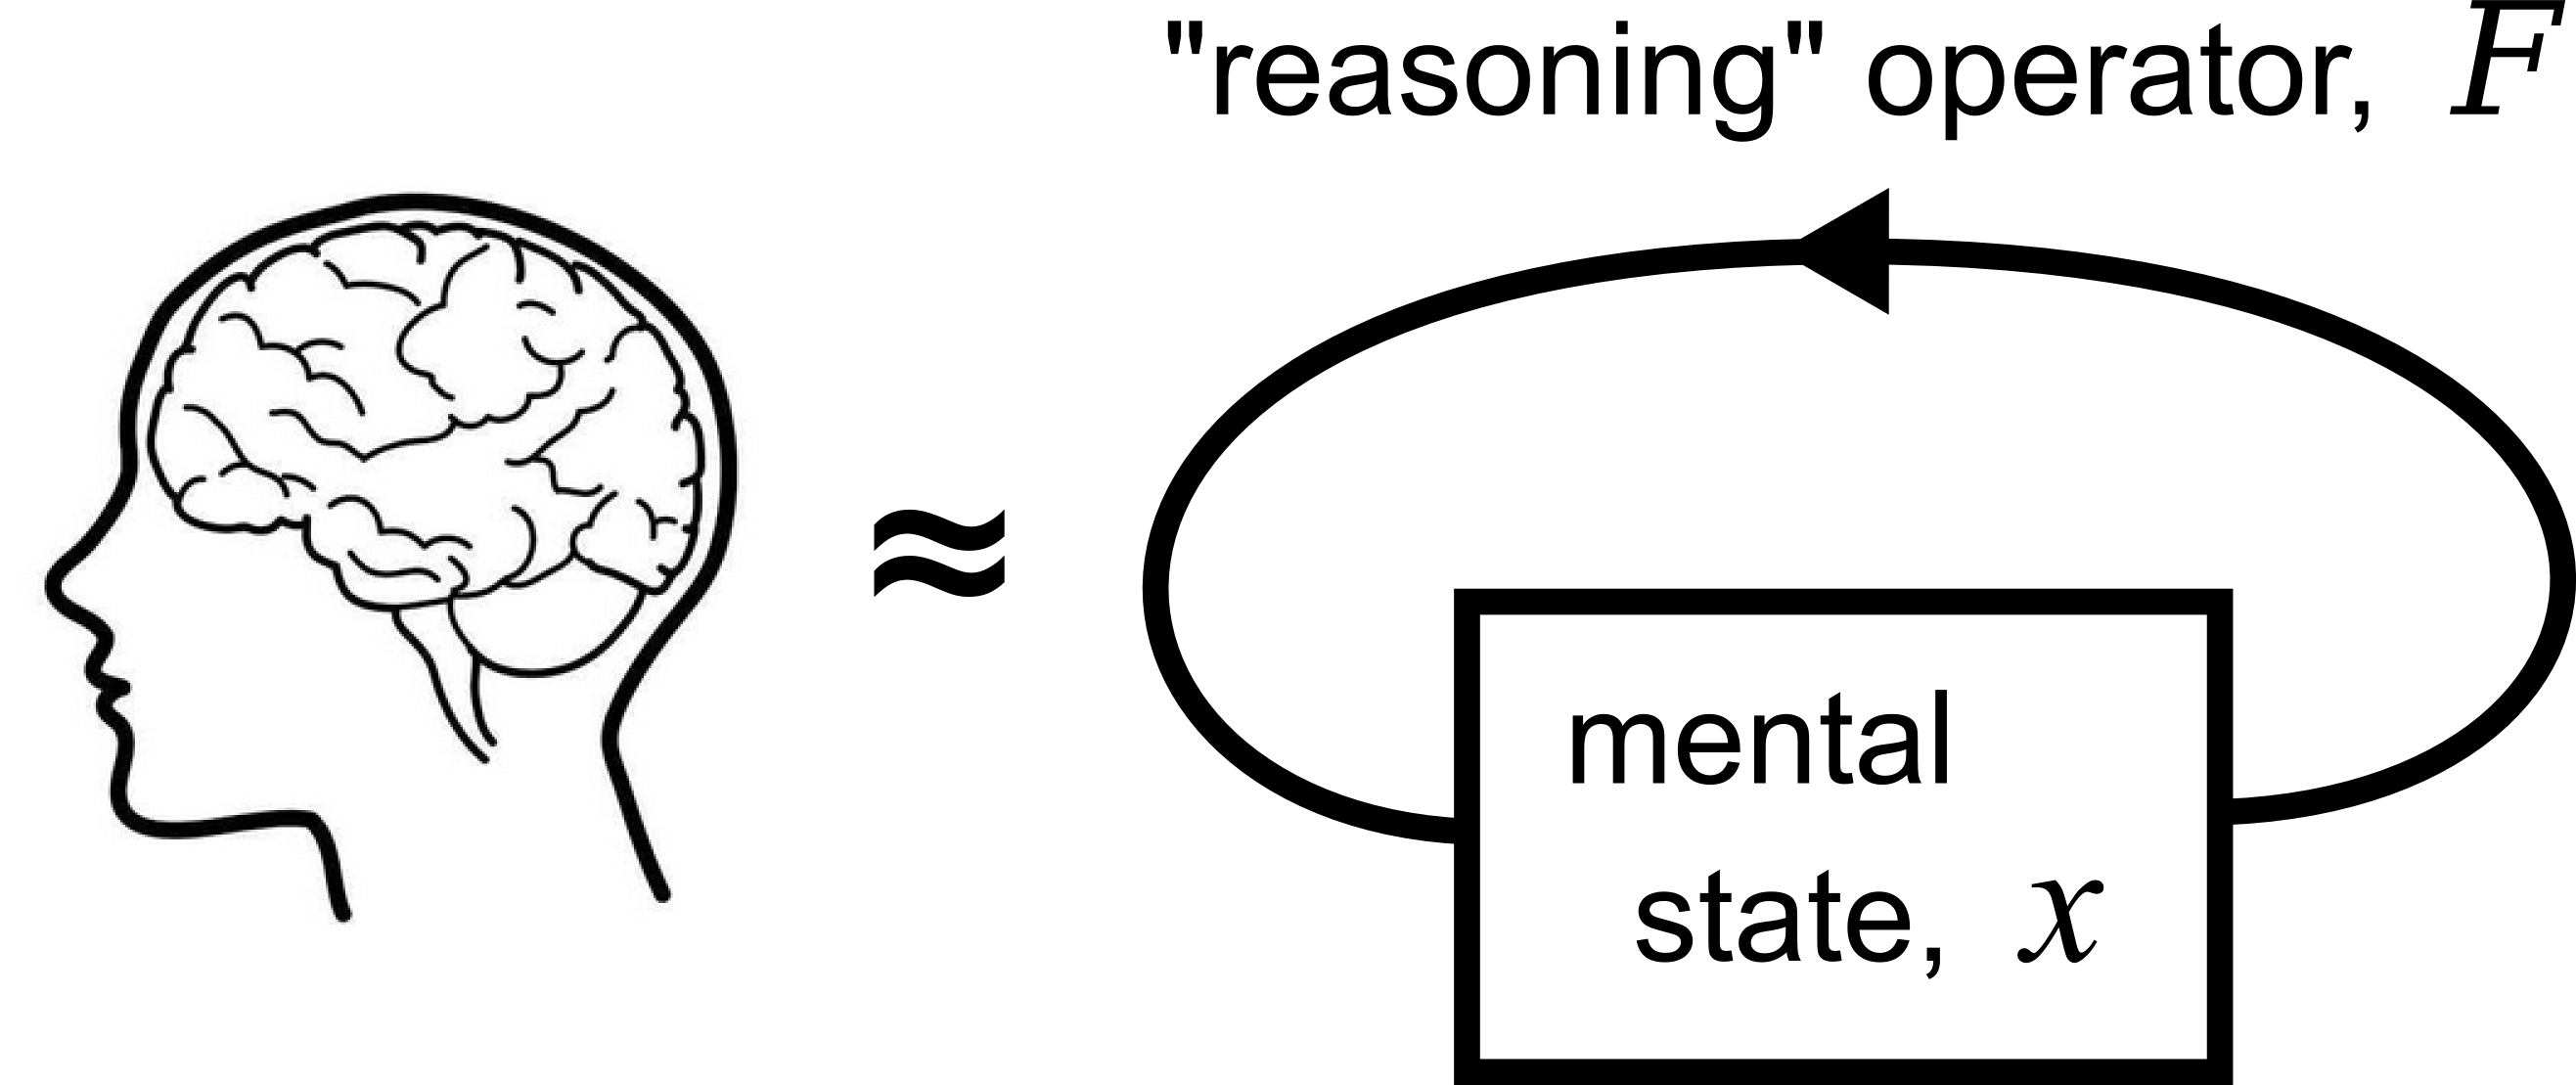
\includegraphics[scale=0.65]{mental-state.png}
\end{equation}

举例来说,一个\emp{思维状态}可以是以下的一束命题:
\let\labelitemi\labelitemii
\begin{itemize}
\item 我在我的房间内,正在写一篇 AGI-17 的论文。
\item 我正在写一句句子的开头:「举例来说,....」
\item 我将会写一个 NP (noun phrase):「一个思维状态....」
\end{itemize}

思考的过程就是从一个思维状态 \emp{过渡} (transition) 到另一个思维状态。 就算我现在说话,我的脑子也是靠思维状态记住我说话说到句子结构的哪部分,所以我才能组织句子的语法。

以下三者其实是同义词:
\begin{itemize}
\item 在人工智能里叫 \textbf{强化学习} (reinforcement learning (RL))
\item 在运筹学里叫 \textbf{动态规划} (dynamic programming)
\item 在现代控制论 (control theory) 中的 \textbf{状态空间}表述
\end{itemize}

\section{控制论:动态系统}

思维状态是一支向量 $\vect{x} \in \mathbb{X}$,$\mathbb{X}$ 是所有可能的思维状态,思考算子 (reasoning operator) $\vect{F}$ 是一个 endomorphism 映射: $\mathbb{X} \rightarrow \mathbb{X}$。

在数学上这是一个标准的\emp{动态系统 (dynamical system)},它可以用以下方法定义:
\begin{eqnarray}
\boxed{\mbox{离散时间}} \quad \quad & \vect{x}_{t+1} = \vect{F}(\vect{x}_t) \label{eqn0}\\
\boxed{\mbox{连续时间}} \quad \quad & \dot{\vect{x}} = \vect{f}(\vect{x}) 
\end{eqnarray}

在我设计的 cognitive architecture 里,$\vect{F}$ 用深度神经网络来表示(所谓「深度」无非是很多层的意思):
\begin{equation}
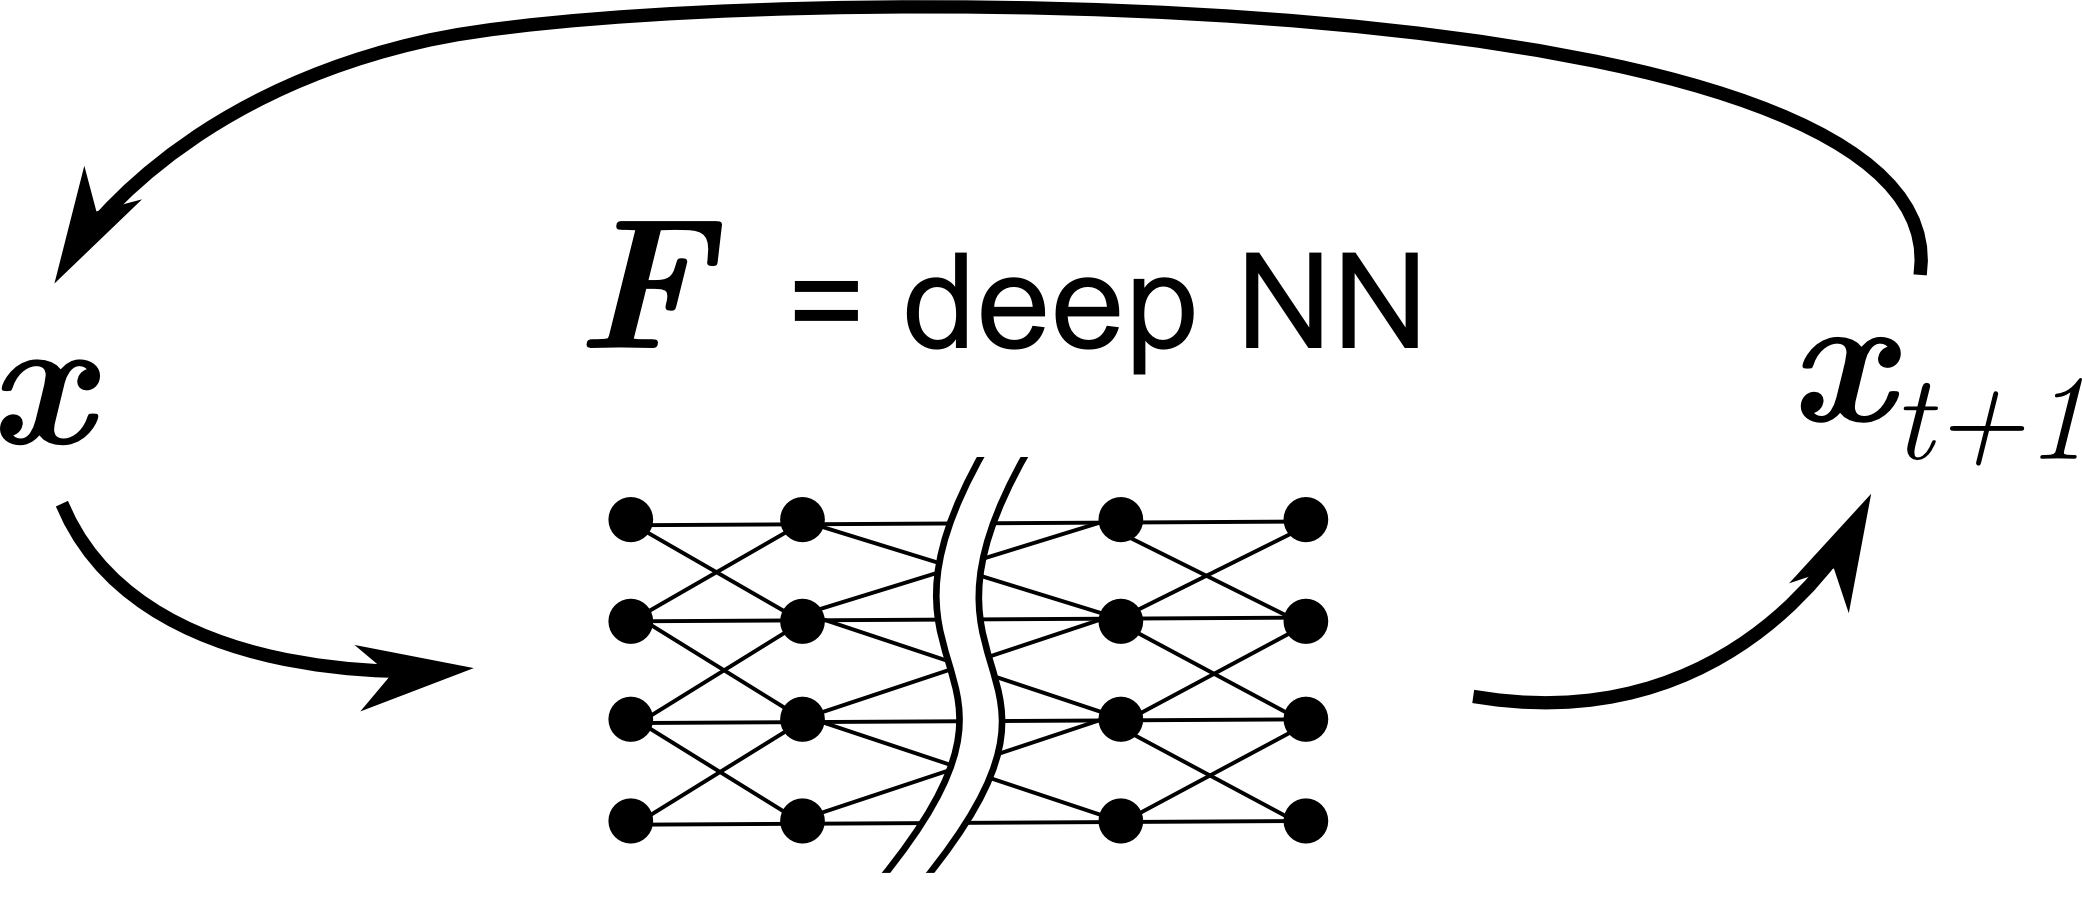
\includegraphics[scale=0.7]{genifer-model-00.png}
\end{equation}
一个\textbf{神经网络}是一个有很多参数的非线性算子:
\begin{equation}
\boxed{\mbox{神经网络} $\; F(\vect{x})$} = \sigmoid(W_1 \sigmoid(W_2 ... \sigmoid(W_L \; \vect{x} )))
\end{equation}
其中 $W_\ell$ 是每一层的\textbf{权重}矩阵,$\sigmoid$ 是一个 sigmoid 形状的非线性函数。 

如果连续时间的话 $\vect{f}$ 也可以用深度神经网络表示,不过这两个 $\vect{F}$ 和 $\vect{f}$ 的性质是不同的,它们之间由这个关系决定: $\vect{x}(t + 1) = \vect{F}(\vect{x}(t))$。 为方便起见,我会随意使用连续或离散时间的表述。

%其中 $f$ 也可以随时间改变。 如果 $f$ 不依赖时间,则系统是 time-invariant (定常的),形式上如(\ref{eqn1}) 那种微分方程叫作 autonomous (自主的)。

%, we would have at disposal all the tools available in vector space such as:

%\begin{itemize}
%\item numerical optimization (including gradient descent)
%\item differential equations governing time evolution
%\item dynamical systems theory, control theory (eg. adaptive filters)
%\item Lie algebra and $C^*$-algebra of continuous operators
%\item matrix theory, iteration and fixed-point theory
%\item dynamic programming (aka. reinforcement learning)
%\item neural networks and deep learning ... etc.
%\end{itemize}

%以下内容可以在一般「现代控制论」教科书中找到,例如:
%\begin{itemize}
%\item Daniel Liberzon 2012: \textit{Calculus of variations and optimal control theory -- a concise introduction}
%\item 李国勇 2008: 《最优控制理论与应用》
%\item 张洪钺、王青 2005: 《最优控制理论与应用》
%\end{itemize}

%在我的智能系统理论里,我把 $F$ 或 $f$ 设定成 RNN (recurrent neural network),即反馈式神经网络:
%\begin{eqnarray}
%\mbox{离散时间:} \quad \quad & \vect{x}_{t+1} = \boxed{\mbox{RNN}}(\vect{x}_t) \\
%\mbox{连续时间:} \quad \quad & \dot{\vect{x}} = \boxed{\mbox{RNN}}(\vect{x})
%\end{eqnarray}
%这里 recurrent 指的是它不断重复作用在 $\vect{x}$ 之上,但实际上它是一个普通的前馈式 (feed-forward) 神经网络。 注意: 在抽象理论中,$f$ 和 $F$ 可以是任意函数,我把它们设计成 NN 只是众多可能的想法之一。 之所以选用 NN,是因为它有 universal function approximator 的功能,而且是我们所知的最「聪明」的学习机器之一。

% Itamar Arel 在 2012 年提出的 \cite{Arel2012}

%在我提出的智能系统里,$\dot{x}$ 是由\emp{學習機器}給出的,換句話說,$\dot{x}$ 是思維狀態在梯度下降至最佳狀態時的\emp{方向導數}。

\emp{控制系统 (control system)} 和动态系统的分别是在定义中加入了 \emp{控制向量}  $\vect{u}(t)$:
\begin{equation}
\dot{\vect{x}}(t) = f(\vect{x}(t), \vect{u}(t), t)
\end{equation}
控制论的目的就是找出最好的 $\vect{u}(t)$ 函数,令系统由初始状态 $\vect{x}_0$ 去到终点状态 $\vect{x_\bot}$。

一个典型的控制论问题是这样描述的:
\begin{eqnarray}
\boxed{\mbox{状态方程}} \quad & \dot{\vect{x}}(t) = \vect{f}[\vect{x}(t), \vect{u}(t), t] \label{eqn1}\\
\boxed{\mbox{边值条件}} \quad & \vect{x}(t_0) = \vect{x}_0 \,,\, \vect{x}(t_\bot) = \vect{x}_\bot \\
\boxed{\mbox{目標函数}} \quad & J = \int_{t_0}^{t_\bot} L[\vect{x}(t), \vect{u}(t), t] dt
\end{eqnarray}
要找的是最优控制 $\vect{u}^*(t)$。

根据控制论,\textbf{最优路径}的条件,是由 Hamilton-Jacobi 方程给出:
\begin{equation}
\boxed{\mbox{Hamilton-Jacobi equation}} \quad
0 = \frac{\partial J^*}{\partial t} + \min_u H
\end{equation}
%\frac{d}{dt} V(x,t) = \min_u \{ C(x,u) + \langle \nabla V(x,t), f(x,u) \rangle \} 

跳过一节之后我会解释 $J$,$L$,和 $H$ 的意义。

\section{强化学习/动态规划}

\textbf{Reinforcement learning} 是机器学习里面的一个分支,特别善於控制一只能够在某个环境下 \emp{自主行动} 的个体 (autonomous agent),透过和 \emp{环境} 之间的互动,例如 sensory perception 和 rewards,而不断改进它的 \emp{行为}。  强化学习最典型的比喻是一隻在迷宫中寻找食物和避开敌人的小昆虫。

一个强化学习的系统由 4 个元素的 tuple 构成
\begin{equation}
\boxed{\mbox{强化学习系统}} \; = (\mbox{States} \ni \vect{x}, \mbox{Actions} \ni \vect{u}, R = \mbox{Rewards}, \pi = \mbox{Policy})
\end{equation}
详细可参阅我写的 《强化学习 tutorial》。

$U$ 是一连串行动的 rewards 的总和:
\begin{equation}
\boxed{\mbox{状态 0 的总价值} $\; U(\vect{x}_0)$} = \sum_t \; \boxed{\mbox{时间 t 时的奖励} $\; R(\vect{x}_t, \vect{u}_t)$}
\end{equation}
例如说,行一步棋的效用,不单是那步棋当前的利益,还包括走那步棋之后带来的后果。  例如,当下贪吃一只卒,但 10 步后可能被将死。  又或者,眼前有美味的食物,但有些人选择不吃,因为怕吃了会变肥。

%一个 state 的效用 U 就是: 假设方案固定,考虑到未来所有可能的 transitions,从这个 state 开始的平均期望的 total reward 是多少 :
%$$ U(S_0) = \mathbb{E}[ \; \sum_{t=0}^{\infty} \; \gamma^t \; R(S_t) \; ] $$

%其中 $\mathbb{E[\;]}$ 代表期望值,$\gamma$ 是 discount factor,例如 0.9 或什么。

\textbf{Dynamic programming} 的中心思想是 \textbf{Bellman optimality condition}。 Richard Bellman 在 1953 年提出这个方程,当时他在 RAND 公司工作,处理的是运筹学的问题。 %他也首先使用了 "curse of dimensionality" 这个术语,形容动态规划的主要障碍。

%考虑的问题是: 要做一连串的 sequential decisions。

Bellman equation 说的是: 「\textbf{如果从最佳选择的路径的末端截除一小部分,馀下的路径仍然是最佳路径。}」
%换句话说,如果一系列的选择 A B C D E.... 是最优的,那么这系列除去开始的 A,那 B C D E.... 系列应用在后继的状态上也是最优的。
%用数学表示:
\begin{equation}
\boxed{\mbox{全路径的价值}} = \max_u \{ \; \boxed{\mbox{在当前状态下选择 $\vect{u}$ 的奖励}} + \boxed{\mbox{馀下路径的价值}} \; \}
\end{equation}
\begin{equation}
\boxed{\mbox{Bellman 方程}} \quad U^*(\vect{x}) = \max_{ \; \vect{u}} \{ R(\vect{u}) + U^*(\vect{x}_{t+1}) \; \}
\end{equation}
%$*$ 表示 \emp{最优} (optimal)。 
这条看似简单的式子是动态规划的\textbf{全部内容}。 它的意义是: 我们想获得最佳效益的路径,所以将路径切短一些,於是问题化解成一个较小的问题;  换句话说它是一个 \textbf{recursive relation}。

在人工智能中常用一个 trick,叫 \textbf{Q-learning}。 $Q$ 值是 $U$ 值的一个变种 ;   $U$ 是对每个 state 而言的,$Q$ 把 $U$ 值分拆成每个 state 中的每个 action 的份量。  换句话说,$Q$ 就是在状态 $\vect{x}$ 做 动作 $\vect{u}$ 的 utility。 $Q$ 和 $U$ 之间的关系是:
\begin{equation}
U(\vect{x}) = \max_{\vect{u}} \; Q(\vect{x}, \vect{u})
\end{equation}
$Q$ 的好处是方便学习,只需要学习在每一个状态下选择哪个动作的价值; 亦即所谓 "model free" 学习。
%$Q$ 的好处是什么?  下面将会介绍 active learning,而 $Q$ value  配合 TD learning,可以在 active learning 中也消除 $P$,达到 model-free 的效果。

%上面的 update rule 只要用这个关系改写就行:
%$$ U(S) \mbox{  +=  } \alpha ( \; R(S) + \gamma \max_{A'}  Q(A', S') - Q(A, S) \; ) $$

%注意: 人工智能中的 \emp{A* search},是动态规划的一个特例。 换句话说,用动态规划在某个空间中「漫游」,可以模拟到 best-first 搜寻的功能。

在强化学习的框架下,智能系统的运作可以分开成两方面: \emp{思考} 和 \emp{学习}。
\begin{itemize}
\item \emp{思考}即是根据已学得的\textbf{知识}(知识储存在 deep NN 里),在思维空间中找寻 $\vect{x}$ 最优的轨迹,方法是根据 Bellman 方程计算 $\vect{u}^*$。 $\vect{x}$ 的轨迹受 deep NN 约束(亦即是说,系统只能依据\textbf{正确的知识}去思考),思考时 deep NN 是\textbf{不变}的。
\item \emp{学习}就是学习神经网络 deep NN 的 weights $W_\ell$,改变 $W$ 即改变 $\vect{F}$,而$\vect{F}$ 决定\textbf{状态方程} (\ref{eqn0}),所以整个系统变了另一个系统。 换句话说,deep NN 的学习是一种 \textbf{second-order learning}: 考虑两个系统 $\vect{F}$ 和 $\vect{F} + \epsilon \vect{F}_0$,经过很多次思考过程,如果奖励的平均值在后者有所增加,则 $\vect{F}$ 向 $\vect{F}_0$ 方向学习。
\end{itemize}

%以上两者是两个独立的方面,但不排除它们可以在实际中同时进行。

\section{控制论与强化学习的关系}

在\emp{强化学习}中,我们关注两个数量:
\let\labelitemi\labelitemii
\begin{itemize}
\item $R(\vect{x}, \vect{u})$ = 在状态 $\vect{x}$ 做动作 $\vect{u}$ 所获得的 \emp{奖励} (reward)
\item $U(\vect{x})$ = 状态 $\vect{x}$ 的 \emp{效用} (utility) 或 \emp{价值} (value) % 或 $V(\vect{x})$
\end{itemize}
简单来说,「价值」就是每个瞬时「奖励」对时间的积分:
\begin{equation}
\boxed{\mbox{价值} U} = \int \boxed{\mbox{奖励} R} \,dt
\end{equation}
%(价值有时用 $V$ 表示,但为避免和势能 $V$ 混淆故不用。)

用\emp{控制论}的术语,通常定义 cost functional:
\begin{equation}
\boxed{\mbox{价钱 } J} = \int L dt + \Phi(\vect{x}_\bot)
\end{equation}
其中 $L$ 是 ``running cost'',即行走每一步的「价钱」; $\Phi$ 是 terminal cost,即到达终点 $\vect{x}_\bot$ 时,那位置的价值。

%Define a continuous version of ``utility'':
%\begin{equation}
%V(x,t) = \min_u \{ \int_t^{t_\bot} C(x,u)dt + \Phi(x_\bot,t_\bot) \} 
%\end{equation}
%where $t$ is time, $u$ is a set of control parameters, $C$ is the \emp{cost-rate} function:
%\begin{equation}
%\int C dt = R = \mbox{reward}
%\end{equation}
%This integral expresses the ``cost of the path'', whereas $\Phi(x_\bot,t_\bot)$ is the ``cost at termination''.

在\emp{分析力学}里 $L$ 又叫 \textbf{Lagrangian},而 L 对时间的积分叫「\textbf{作用量}」:
\begin{equation}
\boxed{\mbox{作用量 (Action) \; S}} = \int L dt
\end{equation}
Hamilton 的\emp{最小作用量原理} (principle of least action) 说,在自然界的运动轨迹里,$S$ 的值总是取稳定值 (stationary value),即比起邻近的轨迹它的 $S$ 值最小。

\textbf{Hamiltonian} 的定义是 $\displaystyle H = L + \frac{\partial J^*}{\partial \vect{x}} \vect{f}$,它是由 Lagrange multiplier 的方法走出来的。 详细可参看我写的《控制论 tutorial》。

其实它们讲的是同一样东西,所以有如下的对应:
\begin{center}
\begin{tabular}{|c|c|c|}
\hline 
\emp{强化学习} & \emp{最优控制} & \emp{分析力学} \\ 
\hline
效用/价值 $U$ & 价钱 $J$ & 作用量 $S$ \\ 
\hline 
即时奖励 $R$ & running cost & Lagrangian $L$ \\ 
\hline 
action $a$ & control $u$ & (外力?) \\
\hline
\end{tabular} 
\end{center}

%用比较浅显的例子: 和美女做爱能带来即时的快感 (= 奖励 $R$),但如果强奸的话会坐牢,之后很长时间很苦闷,所以这个做法的长远价值 $U$ 比其他做法较低,正常人不会选择它。

有趣的是,奖励 $R$ 对应於力学上的 Lagrangian,其物理学单位是「能量」; 换句话说,「快感」或「开心」似乎可以用「能量」的单位来量度,这和通俗心理学里常说的「正能量」不谋而合。 而,长远的价值,是以 $[\mbox{能量} \times \mbox{时间}]$ 的单位来量度。

%一个智能系统,它有「智慧」的条件,就是每时每刻都不断追求「开心能量」或奖励 $R$ 的最大值,但它必需权衡轻重,有计划地找到长远的效用 $U$ 的最大值。

\section{经典逻辑 AI}

在系统的状态方程 (\ref{eqn0}) 中,$\vect{F}$ 是可以自由变动的($\vect{F}$ 代表被学习的知识),换句话说,整个系统几乎没有结构。 在无限维的泛函空间搜寻 $\vect{F}$ 是不切实际的,所以要引入逻辑 AI 的结构,令 $\vect{F}$ 的搜寻範围缩小。 在机器学习中这种做法叫 inductive bias,是加快学习的必经之路。 这个问题会在我的论文《神经与逻辑之间的桥》探讨(先前发表了初稿,但那里有不少漏洞)。

换句话说: 我们的目的是想将整套逻辑 AI 的器材搬到 \emp{连续} 的微分流形上去实现。  这个做法,是受了 Google 的 Word2Vec \cite{Mikolov2013} 算法的启发,它可以将自然语言的词语 embed 到度量空间中,而且词语之间的距离是 \emp{semantic distance} (\textbf{语义学上的距离}):
\begin{equation}
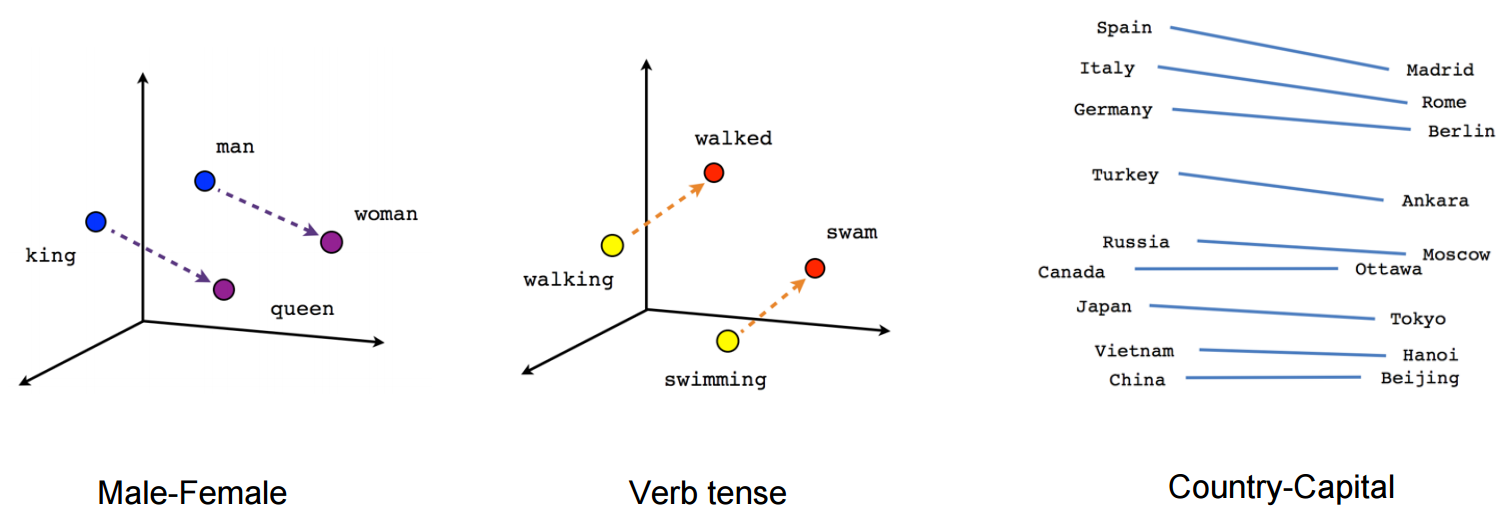
\includegraphics[scale=0.3]{word2vec-relations.png}
\end{equation}
当然,word2vec 一经发表之后,很多人开始构思怎样把「句子」也 embed 到度量空间上。 第一个想法当然是用 \textbf{tensor product},例如 ``he loves her'' 这句子就变成了 $\mbox{he} \otimes \mbox{loves} \otimes \mbox{her}$。 但这个做法很有问题; 例如『人不可貌相』和『金玉其外~ 败絮其中』这两句句子意义相近,但表面上 (syntax) 却很不同。 用 tensor product 的做法,得出的空间结构是 syntactic 而不是 semantic 的,但神经网络学习的重点是 \emp{泛化} (generalization),它基於「邻近的点的意义相近」才能成功,所以一定要 semantic distance。

有一个新的想法是: 不要看状态空间 $\mathbb{X}$ 的结构,因为这牵涉到逻辑原子概念怎样组合成逻辑句子的 composition 问题,这 composition 如果是 algebraic 的就会产生上面的 syntactic 问题。 解决办法是: 考虑 $\mathbb{X} \rightarrow \mathbb{X}$ 之间的\textbf{函数}。 这些函数的 \emp{环} 反过来决定 $\mathbb{X}$ 的结构。 Nestruev 2003 的书《Smooth Manifolds and Observables》有讲述类似的观点。

换句话说,$\vect{F}: \mathbb{X} \rightarrow \mathbb{X}$ 应该由两个\textbf{家族合并}而成: 一个是根据 Bellman 的学习算子,另一个是逻辑的学习算子。

\begin{comment}
% ===========================================================================

换句话说: 我们的目的是想将整套逻辑 AI 的器材搬到向量空间中去实现。 这个做法,部分是受到 Google 的 PageRank \cite{Page1999} 和 Word2Vec \cite{Mikolov2013} 算法的启发,因为它们都是在向量空间中运作,而且非常成功。 %, both exploit the efficiency of vector and matrix calculus.

Strong AI 的问题在理论上已经被\emp{数理逻辑}完整地描述了,馀下的问题是\emp{学习算法},因为在逻辑 AI 的架构下,学习算法很慢(复杂性很高),这就是我们要解决的。

我研究 logic-based AI 很多年,因此我的思路喜欢将新问题还原到逻辑 AI 那边去理解,但实际上我提倡的解决办法不是靠经典逻辑,甚至不是 symbolic 的。  但在这篇文章我还是会经常跳回到逻辑 AI 去方便理解。

用数理逻辑模拟人的思想是可行的,例如有 deduction, abduction, induction 等这些模式,详细可见《Computational logic and human thinking》by Robert Kowalski, 2011.  这些方面不影响本文的阅读。 值得一提的是,作者 Kowalski 是 logic programming,特别是 Prolog,的理论奠基人之一。

在经典逻辑 AI 中,「思考」是透过一些类似以下的步骤:
\begin{eqnarray}
\mbox{前提} & \vdash & \mbox{结论} \\
\boxed{\mbox{今天早上下雨}} & \vdash & \boxed{\mbox{草地是湿的}}
\end{eqnarray}
亦即由一些\emp{命题}(propositions)推导到另一些命题。

推导必须依靠一些逻辑的法则命题 (rule propositions),所谓「法则」是指命题里面带有 x 这样的\emp{变量}(variables):
\begin{equation}
\boxed{\mbox{地方 x 下雨}} \wedge \boxed{\mbox{x 是露天的}} \vdash \boxed{\mbox{地方 x 是湿的}}
\end{equation}
这些法则好比「逻辑引擎」的燃料,没有燃料引擎是不能推动的。

注意: 命题里面的 x,好比是有「洞」的命题,它可以透过 substitution 代入一些实物 (objects),而变成完整的命题。 这种「句子内部」(sub-propositional)的结构可以用 predicate logic (谓词逻辑)表达,但暂时不需要理会这些细节。

Logic-based AI 可以看成是将世界的「模型」压缩成一个「知识库」(knowledge-base, KB),里面装著大量逻辑式子:
\begin{equation}
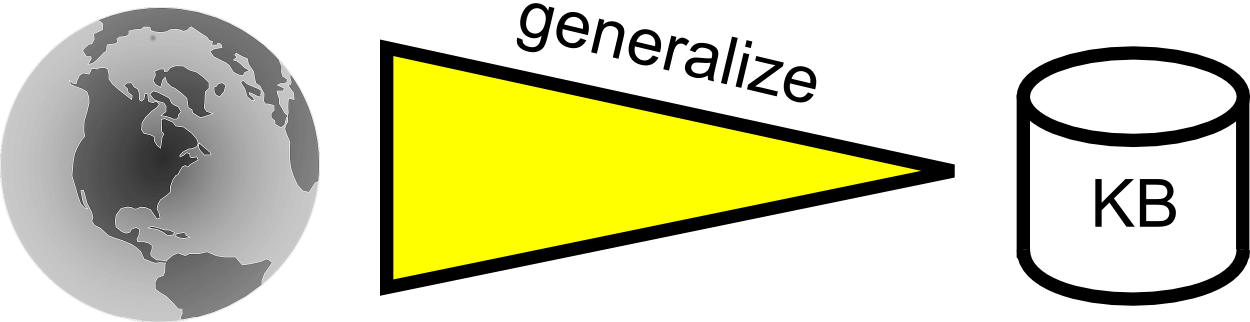
\includegraphics[scale=0.5]{world-model-compression.png}
\end{equation}
世界模型是由大量的逻辑式子经过组合而\emp{生成}的,有点像向量空间是由其「基底」生成; 但这生成过程在逻辑中特别复杂,所以符号逻辑具有很高的\emp{压缩比},但要学习一套逻辑知识库,则相应地也有极高的\emp{复杂度}。

\end{comment}
% ===========================================================================

\section{Episodic memory}

设计了这个 minimalist architecture 之后,发现比较起人脑有个严重缺陷: 没有 \emp{事件记忆} (episodic memory)。 换句话说,只能留意\textbf{当下}发生的事件,但不能记住一段\textbf{故事}。

这牵涉到「什么是记忆?」的问题。 在 minimal architecture 里,$\vect{F}$ 代表 ``static knowledge'',亦即(相对地)\textbf{永恒不变}的知识/规律,而 $\vect{x}$ 代表当下的\textbf{状态}/短期记忆,亦即 ``dynamic knowledge''。  Episodic memory 介乎「长期」与「短期」记忆之间。

\textbf{深度学习} 在近年很厉害,但 deep NN 的缺点是没有\textbf{记忆}。 有限自动机 (finite state machines) 不是\textbf{全能}的计算器,它和 Turing machine 的分别就是缺少了那条「记忆磁带」。 所以,深度神经网络 + 记忆~ 就可以变成 universal 的计算器。 如何设计「可微分」的记忆是一重要课题,因为可微分的记忆可以用 gradient descent 学习。 

在 \textbf{信息处理} (signal processing) 理论中,$z$-transform 以 $z^{-1}$ 可以代表 \textbf{时间延迟} 1 步 (1-step time delay unit)。 用一连串的 $z^{-1}$ 可以组成长度为 $k$ 单位的记忆:
\begin{equation}
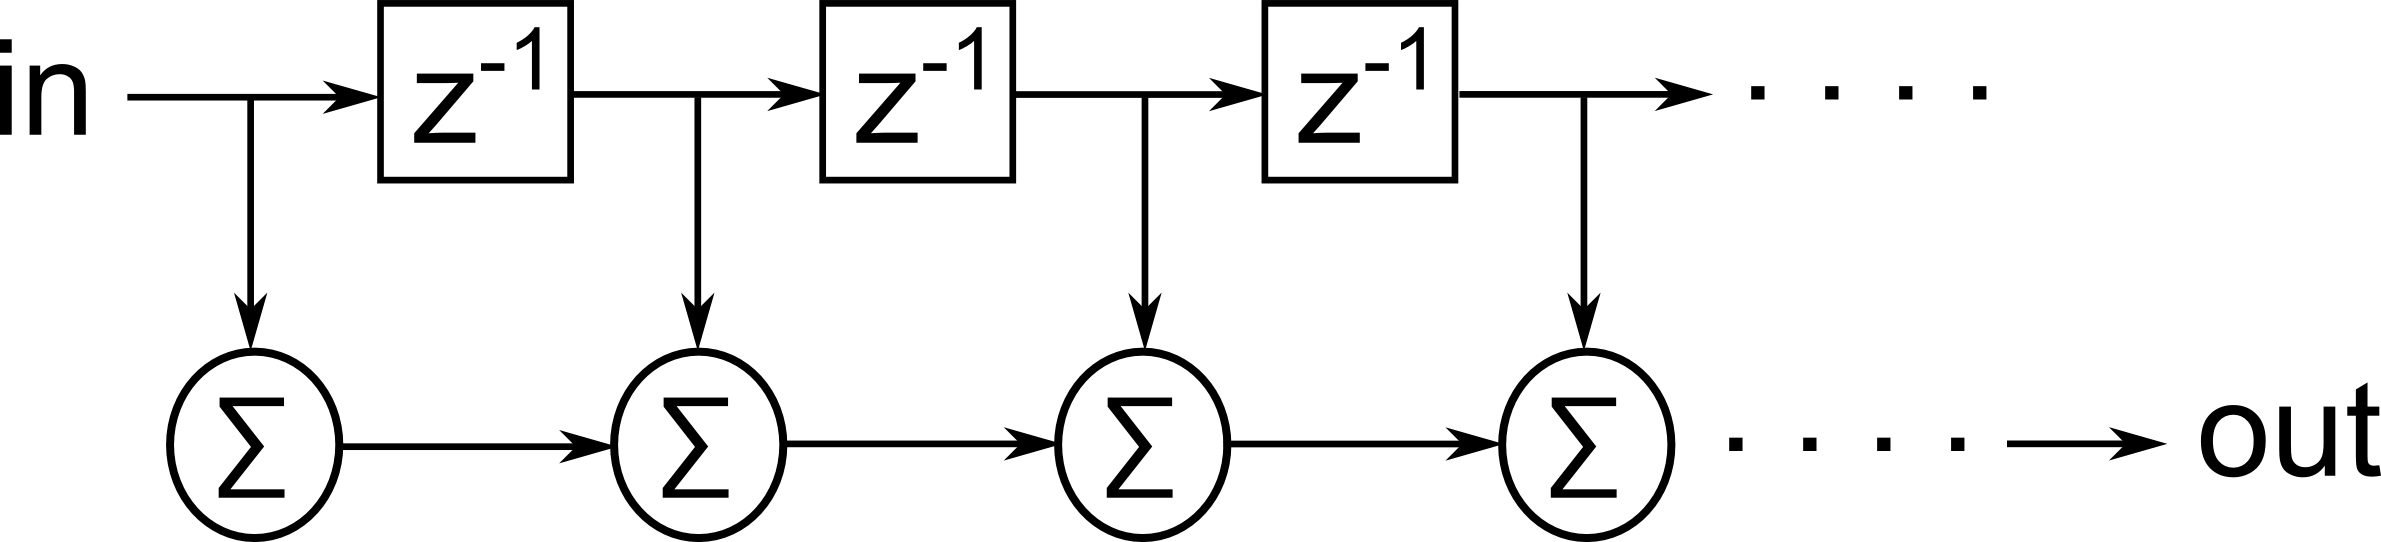
\includegraphics[scale=0.9]{z-memory-0.png}
\end{equation}
以上的无穷串列可以用这个 recursive 结构代替:
\begin{equation}
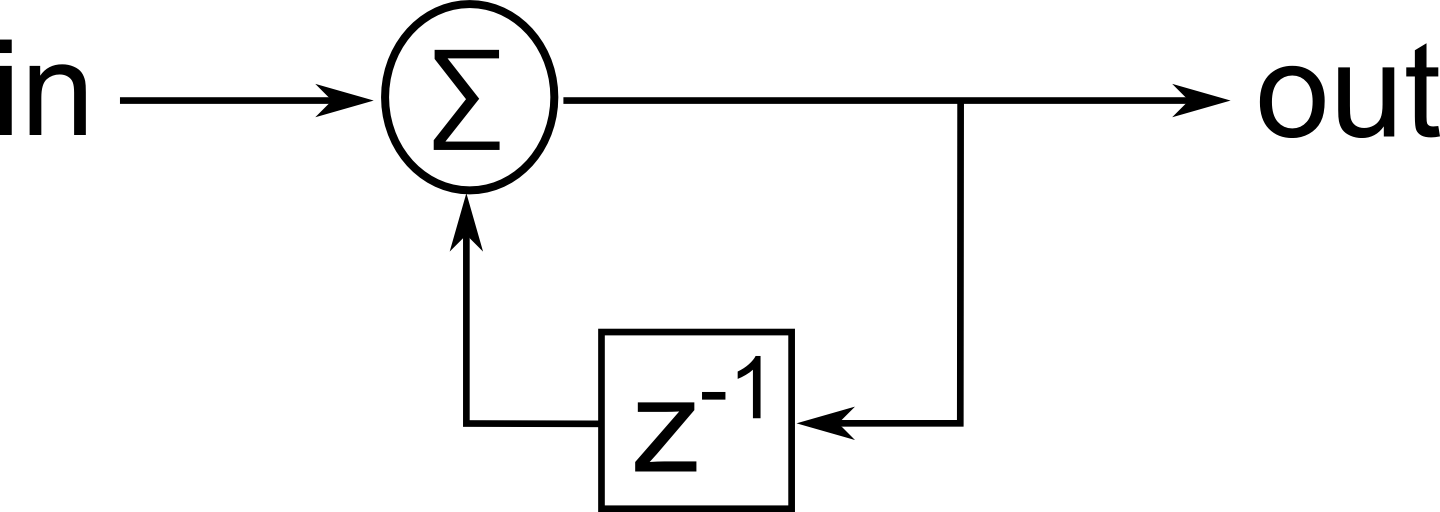
\includegraphics[scale=0.9]{z-memory-1.png}
\end{equation}
多层的 hierarchical 记忆可以这样实现:
\begin{equation}
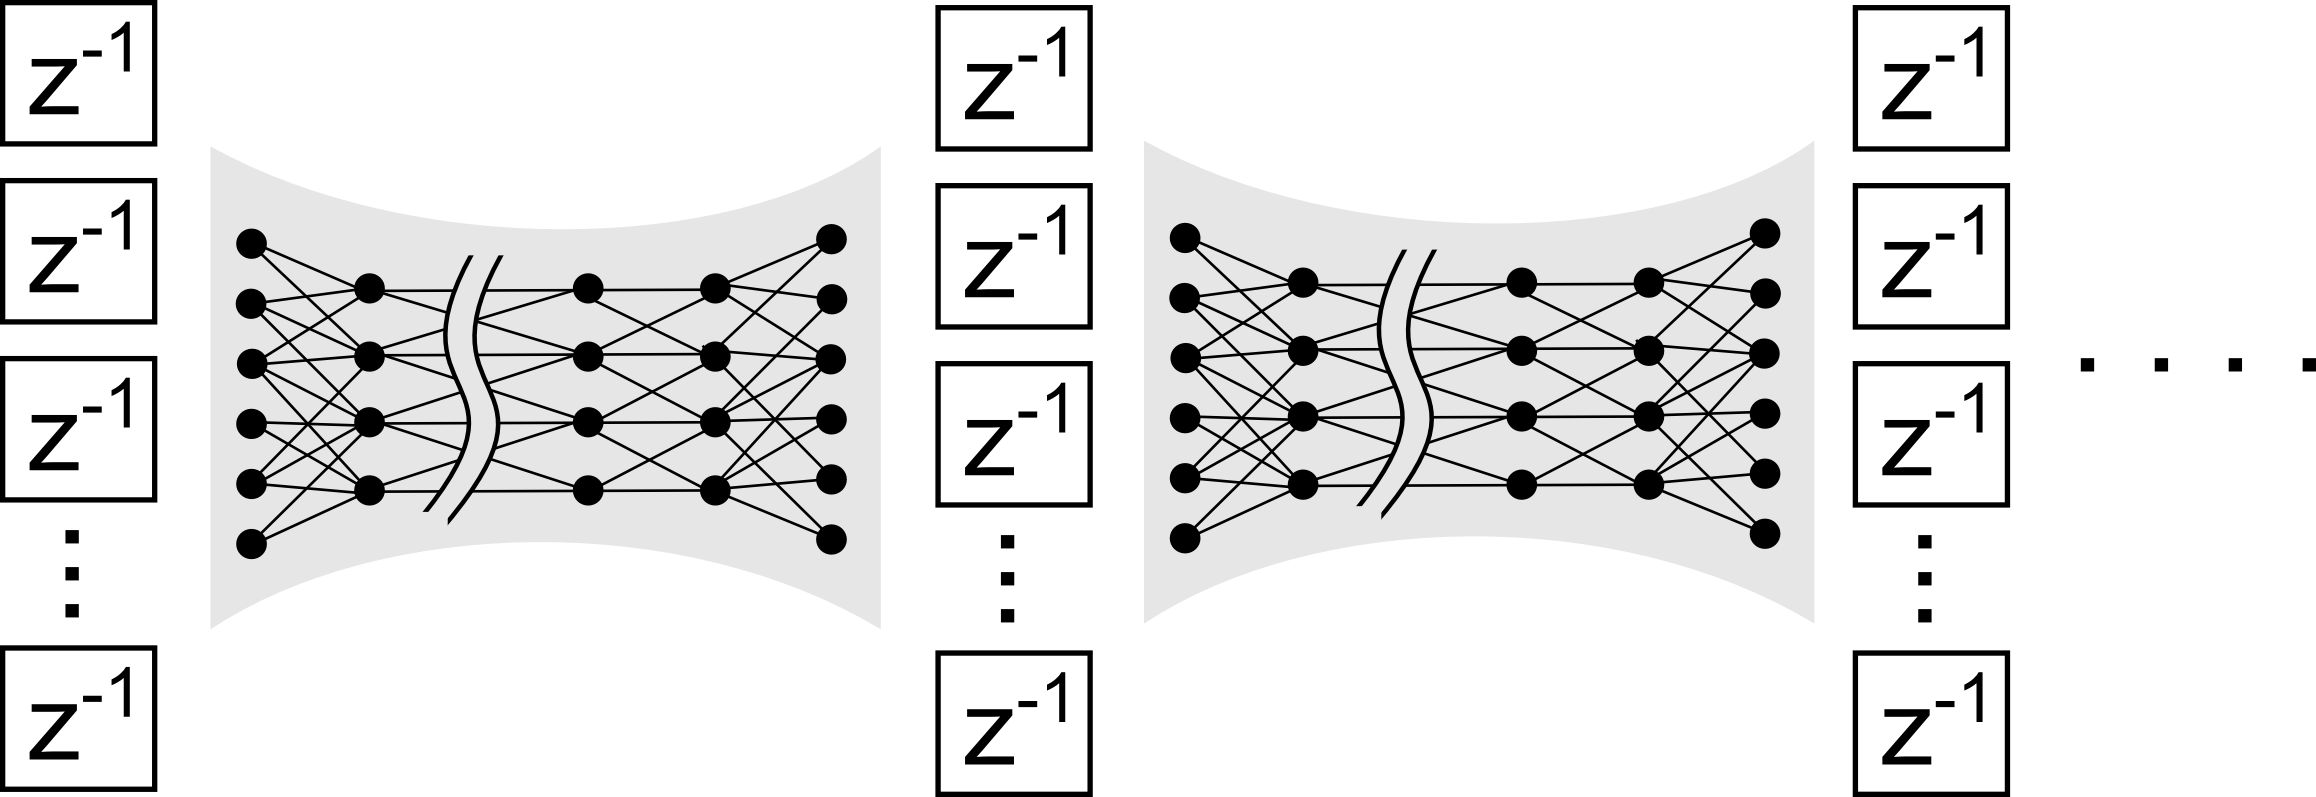
\includegraphics[scale=1.0]{z-memory-2.png}
\end{equation}
Z-transform 的\textbf{连续时间}版本就是 Laplace transform。

信号处理的资深研究者 Simon Haykin 最近也用 RL + 记忆~ 的设计,详见他的 2012 新书 《Cognitive dynamic systems》。 

%\section*{Acknowledgements}

%\footnotesize{In a forum discussion with Ben Goertzel dated 25 June 2014 on the AGI mailing-list: (artificial-general-intelligence @googlegroups.com), YKY asked: Why bother with neural networks, which typically require many neurons to encode data, when logic-based AI can represent a proposition with just a few symbols?  Ben's insight is that neural networks are capable of learning its own representations, and their learning algorithms are relatively fast.  We have been working on "neo-classical" logic-based AI for a long time, and begin to realize that inductive learning in logic (based on combinatorial search in a symbolic space) is perhaps \textit{the bottleneck} in the entire logic-based paradigm.  So we try to look for alternatives that might enable learning to be faster, though we would still emphasize that logic-based AI remains a viable approach to AGI. %, provided that the right search heuristics be found (most probably in the form of \emp{hierarchical organization} of the learning space).}

\bibliographystyle{plain} % or number or aaai ...
\bibliography{AGI-book}

\end{document}
